%% ------------------------------------------------------------------------- %%
\chapter{Arquitetura para a Distribuição do Processamento de Eventos Complexos}
\label{cap:arquitetura}

Com o objetivo de criar um sistema auto-escalável para o processamento de dados de cidades inteligentes em tempo real, este trabalho de mestrado propõe uma arquitetura de microsserviços para a execução e distribuição do processamento de eventos complexos.

As seções a seguir descrevem os componentes da arquitetura e os mecanismos de distribuição.

\section{Arquitetura CEP Handler}
 %Estes dados são transformados em eventos, que podem ser usados como entrada para tipos de eventos definidos pelo usuário. Para um usuário ser notificado da ocorrência de um evento, ele pode cadastrar um \textit{webhooks}, uma URL para ser chamada por API REST, o sistema enviará o evento em formato JSON para o usuário por método POST
Essa arquitetura, chamada \texttt{CEP Handler}, consiste em quatro microsserviços -- \texttt{CEP Cataloger}, \texttt{Event Composer}, \texttt{Event Sender} e \texttt{CEP Worker} -- e utiliza mais dois microsserviços prontos para realizar sua funções: um sistema gerenciador de bancos de dados chave-valor e um sistema de mensageria. Todos esses microsserviços operam sob um serviço de gerenciamento dinâmico de recursos na nuvem. 
A Figura \ref{fig:system_architecture} mostra os componentes da arquitetura \texttt{CEP Handler}. A arquitetura foi desenhada com o intuito de estender a plataforma InterSCity de cidades inteligentes, recebendo dados em tempo real dela. 

\begin{figure}[hb]
      \centering
      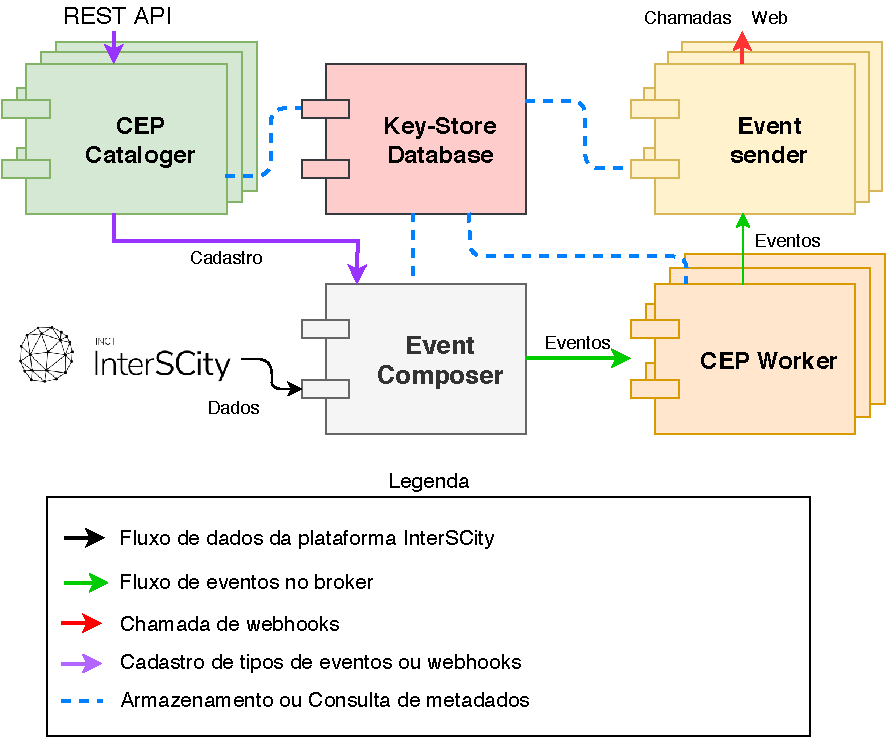
\includegraphics[width=0.7\textwidth]{figuras/neopr.pdf}
      \caption{Arquitetura \texttt{CEP Handler} para processamento distribuído de eventos complexos.}
      \label{fig:system_architecture}
\end{figure}

%\todo[inline]{Fernando, este é o capítulo no qual você começa a apresentar sua solução. Antes sair explicando cada microsserviços separadamente, você primeiro precisa retomar aqui qual é o problema alvo do seu trabalho e o seus objetivos quanto a ele, e depois dar uma visão geral (de alto nível) da solução que você está propondo. Só depois disso você pode começar a detalhar os microsserviços, caso contrário o leitor do texto já começará o capítulo 4 perdido! Sugiro que você apresente a figura da arquitetura aqui no começo do capítulo. E acho que dá pra aproveitar aqui trechos que foram escritos no artigo do ERAD.}
%Neste capítulo, é apresentada a arquitetura de microsserviços proposta para distribuir o processamento de eventos complexos, chamada de \texttt{CEP Handler}. Ela consiste em quatro microsserviços: \texttt{CEP Cataloger} (Seção \ref{sec:cepcataloger}), \texttt{Event Composer} (Seção \ref{sec:eventcomposer}), \texttt{Event Sender} (Seção  \ref{sec:eventsender}) e \texttt{CEP Worker} (Seção \ref{sec:cepworker}).



%\todo[inline]{A figura da arquitetura não mostra que é possível ter múltiplas instâncias de um CEP Worker. Ela deveria mostrar. Na figura, trocar "web hook" por "webhook" (se escreve tudo junto).}

\subsection{Microsserviço CEP Cataloger} \label{sec:cepcataloger}

O microsserviço \texttt{CEP Cataloger} é responsável por prover uma API RESTful para o usuário cadastrar novos tipos de eventos para serem detectados e \textit{webhooks}, que são URLs a serem chamadas pelo sistema por REST quando eventos de tipos cadastrados forem detectados. Ele disponibiliza seis funcionalidades principais para o usuário:
\begin{itemize}
    \item Cadastrar um novo tipo de evento: o usuário pode cadastrar novos tipos de eventos no sistema para que sejam detectados. Como a fonte de dados é a plataforma InterSCity%\todo{!!! Observe que você não falou ainda no texto qual é a relação do \texttt{CEP Handler} e a plataforma InterSCity. Você precisará falar sobre isso na introdução do capítulo.}
    , o usuário deve fornecer os identificadores dos recursos e capacidades cadastrados na plataforma ou os identificadores de outros tipos de eventos já cadastrados para servirem como origem dos eventos de entrada, além de um nome e uma definição para o novo tipo de evento, descrevendo que processamento deve ser feito.
    \item Listar eventos cadastrados: o usuário pode verificar quais tipos de eventos já estão cadastrados, para poder utilizá-los como tipos de entrada ou associar \textit{webhooks} a eles.
    \item Cadastrar \textit{webhooks}:  o usuário pode cadastrar endereços URL para servirem como \textit{webhooks}, fornecendo o identificador de um tipo de evento e o endereço URL associado a ele. Cada vez que o evento desse tipo for detectado, uma chamada será feita para o URL, pelo \texttt{Event Sender}, passando os dados do evento detectado.
    \item Listar \textit{webhooks}: o usuário pode ver todos os \textit{webhooks} associados a cada um dos tipos de eventos.
    \item Remover \textit{webhooks}: o usuário pode remover um \textit{webhook} associado a qualquer um dos tipos de eventos.
\end{itemize}

\subsection{Microsserviço Event Composer} \label{sec:eventcomposer}
O microsserviço \texttt{Event Composer} é responsável por transformar os dados em tempo real vindos da plataforma InterSCity em eventos de entrada primários, além de ser responsável por cadastrar tipos de eventos de entrada primários. A plataforma InterSCity utiliza o conceito de Recurso para definir objetos espalhados pela cidade que funcionam como sensores ou atuadores e o conceito de Capacidade como os tipos de medições que os Recursos com capacidades sensoriais podem coletar. Quando um usuário cadastra um novo tipo de evento no \texttt{CEP Handler} que utiliza diretamente os dados da plataforma como fonte, ele precisa passar quais Recursos e quais Capacidades desses recursos medem os dados em tempo real%\todo{"Recurso" e "capacidade" são conceitos da plataforma do InterSCity. Para que o leitor possa entender este trecho, você precisa explicar a plataforma antes.}
. O \texttt{Event Composer} cria um tipo de evento primário, que contém como campos de atributos todos os dados da capacidade e recursos especificados. 
Como a plataforma InterSCity transmite internamente os dados em tempo real por meio de um \textit{broker} de mensagens, o \texttt{Event Composer} se inscreve %\todo{se inscreve onde? precisar explicar que a plataforma interscity usa um broker de mensagens, onde publica os dados dos recursos em diferentes tópicos}
para receber os dados das capacidades em tempo real na plataforma. Quando esses dados chegam, ele adiciona as informações dos recursos que originaram os dados e converte-os em formato de evento para que o \texttt{CEP Worker} consiga reconhecer e processar.
%MENCIONAR QUE FOI DESENVOLVIDO PELA UFBA - INSTERSCITY 

\subsubsection{Sistema de Mensageria}
\label{sec:messaging-system}
Para o envio de dados em tempo real entre os microsserviços do sistema \texttt{CEP Handler}, escolheu-se um sistema de mensageria do tipo \textit{broker} de mensagens. Um \textit{broker} de mensagens é definido como um sistema que centraliza o envio e recebimento de mensagens entre serviços, permitindo que qualquer serviço se inscreva para receber mensagens de qualquer outro serviço, no estilo de comunicação assíncrona , como descrito na Seção \ref{sec:servicecom}. Todas os envios de eventos entre os microsserviços desenvolvidos para o sistema \texttt{CEP Handler} são feitos de forma assíncrona por meio do \textit{broker}. 


\subsection{Sistema Gerenciador de Banco de Dados Chave-Valor}
\label{sec:key-value-sgbd}
Para o armazenamento de metadados dos tipos de eventos, como nome, definição em EPL, tipos de eventos de entrada e armazenamento dos \textit{webhooks} associados a cada tipo de evento, optou-se pelo uso de um sistema gerenciador de banco de dados chave-valor. Esta escolha se deve principalmente a esse tipo de SGBD oferecer as menores latência de consulta e escrita em comparação a outros tipos de SGBDs NoSQL ou relacionais. 

\subsection{Microsserviço Event Sender} \label{sec:eventsender}

O \texttt{Event Sender} é responsável por fazer requisições para os \textit{webhooks} cadastrados. 
Ele se inscreve com o \textit{broker} %\todo{que broker? Você não falou sobre brokers antes no texto. Você precisa explicar o que um sistema desse tipo faz e como ele está sendo usado no seu sistema.} 
para receber os tipos de eventos que têm \textit{webhooks} associados e envia uma chamada REST do tipo POST para o endereço, contendo os atributos recebidos em cada evento do tipo associado. Periodicamente, ele consulta o banco de dados chave valor e atualiza a lista de \textit{webhooks} associados.
%\todo[inline]{Fernando, observe que nas explicações acima você menciona "o broker" e o "banco de dados" como seja já tivesse falado sobre a existência deles no seu sistema, mas não falou. Como eles voltam a aparecer nas explicações na sequência do texto, você precisa falar de que se tratam ainda no início do capítulo.}

\subsection{Microsserviço CEP Worker} \label{sec:cepworker}

O \texttt{CEP Worker} é o microsserviço responsável pela detecção contínua de eventos, de forma que cada instência dele pode realizar a detecção de vários tipos de eventos concomitantemente.
Em contraste com os outros microsserviços do \texttt{CEP Handler}, o \texttt{CEP Worker} precisa manter um estado de execução para a detecção de eventos, pois provê a execução de operadores de CEP como Agregação, Composição e Detecção de Padrão, que utilizam dados de vários eventos, como visto na Seção \ref{sec:CEPstate}. Para que a detecção de eventos ocorra da maneira esperada, é necessário que o próprio \texttt{CEP Worker} administre seu uso de recursos computacionais, caso contrário uma sobrecarga levaria a terminação do processo de eventos e a perda do estado de agregação dos tipos de eventos em detecção.


%para que seu processo de execução não sobrecarregue os recursos computacionais e o microsserviço seja terminado.\todo{Não está claro porque ele seria terminado pelo SO caso não administrasse os seus recursos.}. 


Diferentemente do \texttt{CEP Worker}, os outros três microsserviços do sistema \texttt{CEP Handler} não armazenam estado durante seu funcionamento, podendo ser escalados horizontalmente a partir da instanciação de réplicas. %A \autoref{fig:system_architecture} mostra a arquitetura do sistema, com os fluxos de dados e o cadastro de tipos de eventos.

%TROCAR POR VETORIAL


%A \autoref{fig:system_architecture} ilustra a arquitetura do sistema \texttt{CEP Handler}. Conforme já descrito, o microsserviço \texttt{CEP Cataloger} provê uma API RESTful para que o usuário possa interagir com o sistema. Quando um novo tipo de evento que usa dados da plataforma InterSCity é cadastrado, o \texttt{CEP Cataloger} envia uma chamada para o \texttt{Event Composer} criar o tipo de evento de entrada, armazená-lo no banco de dados chave-valor do sistema e começar a receber os dados da plataforma em tempo real, convertendo-os em eventos de entrada. Um \texttt{CEP Worker} consulta o banco de dados chave-valor, toma ciência da criação de um novo tipo de evento, inicia o processo de detecção dele e se inscreve no \textit{broker} para receber os eventos do \texttt{Event Composer} ou de outros \texttt{CEP Workers} para que os eventos comecem a ser detectados, consultando os metadados no banco de dados chave-valor, como nome do tipo de evento e definição. O \texttt{Event Sender} consulta o banco de dados chave-valor para encontrar todos \textit{webhooks} cadastrados no sistema e se inscreve no \textit{broker} para receber os eventos dos tipos que têm \textit{webhooks} associados. Quando estes chegam ao \texttt{Event Sender}, ele converte os eventos em chamadas POST e as envia para os endereços URL associados. 
\subsubsection{Cadastro de novos tipos de evento}
Os passos para o cadastro de novos tipos de eventos podem ser descritos na seguinte ordem:

\begin{enumerate}
    \item O usuário registra os metados do tipos de evento no \texttt{CEP Cataloger}, que por sua vez armazena-os no Banco de Dados.
    \item Caso o tipo de evento cadastrado use os dados da plataforma InterSCity diretamente, o \texttt{CEP Cataloger} envia uma chamada para o \texttt{Event Composer} criar o tipo de evento de entrada, armazená-lo no banco de dados chave-valor do sistema.
    \item o \texttt{Event Composer} realiza a ação anterior e começa a receber os dados da plataforma em tempo real, convertendo-os em eventos de entrada para o novo tipo de evento cadastrado pelo usuário.
    \item Periodicamente, os \texttt{CEP Workers} verificam o banco de dados para o cadastro e início de detecção de novos tipos de eventos. Quando o novo tipo de evento é cadastrado, o \texttt{CEP Worker} se inscreve no \textit{broker} para receber os eventos de entrada gerados pelo \texttt{Event Composer}.
    \item Periodicamente, o \texttt{Event Sender} atualiza sua lista interna de \textit{webhooks} a serem chamados na detecção de cada tipo de evento e se inscreve no \textit{broker} para receber os tipos de evento com \textit{webhooks} associados.
    \item Quando o \texttt{CEP Worker} detecta um evento do novo tipo de evento, o evento é enviado ao \textit{broker} e chega ao \texttt{Event Sender} que o converte em chamada POST e o envia para os endereços URL associados.
\end{enumerate}


%\todo[inline]{Na explicação acima, sobre o funcionamento geral do CEP Handler, seria melhor dividir o texto em uma lista de passos numerados ou no formato de algoritmo, ficaria mais fácil de entender.}

%\todo[inline]{É preciso dizer que uma instância de CEP Worker pode ser responsável pela detecção de vários tipos de eventos ao mesmo tempo.}


\subsubsection{Funcionamento do CEP Worker}
\label{sub-sec:cep-worker-func}

O \texttt{CEP Worker} é o principal microsserviço do sistema \texttt{CEP Handler}. Além de ser responsável pelo processamento dos tipos de eventos, ele tem a capacidade de auto-escalabilidade horizontal, a partir da criação de novas instâncias de si próprio. Para distribuir o processamento de eventos entre as instâncias, o \texttt{CEP Worker} utiliza uma série de técnicas para selecionar qual tipo de evento será realocado, como é feita a realocação do tipo de evento sem perda de detecção a partir dos eventos de entrada e como é feito o monitoramento do uso de recursos. O \texttt{CEP Worker} utiliza o SGBD chave-valor para compartilhar todos os dados que são utilizados por mais de uma instância, como metadados de tipos de eventos, informações sobre a realocação de tipos de eventos, etc. 

O disparo da criação de novas instâncias do \texttt{CEP Worker} é feito a partir do monitoramento de recursos (CPU e memória) utilizados por cada instância. São definidos dois limites de sobrecarga, um limite fraco e outro forte. Quando o limite fraco é atingido, a instância pára o cadastramento de novos tipos de eventos para processamento e mantém o processamento dos tipos de eventos já cadastrados. Quando o limite forte é atingido, a instância inicia o processo de realocação dos tipos de evento. A partir do momento em que é iniciada, cada instância nova do \texttt{CEP Worker} recebe um identificador e inicia três \textit{threads}, cada um com uma responsabilidade distinta: 

%\todo[inline]{Aqui, é bom começar a seção com algumas explicações mais gerais sobre os Workers, para a ajudar o leitor a entender mais facilmente a descrição "mais baixo nível" que vem a seguir. É bom explicar que os workers são auto-escaláveis e responsáveis pelo balanceamento da carga, que se comunicam por meio do banco de dados, etc. Explicar também  que o sistema cresce quando o consumo de recursos em todos os workers fica acima de um limite pré-definido,  e diminui quando ... Dizer que há dois limites de sobrecargas considerados num worker: um para impedir novas alocação de tipos no worker (o fraco) e outro para iniciar a redistribuição de tipos já alocados nele (forte). }


\begin{itemize}
   
\item O \textit{thread} de Aceitação é responsável pelo cadastro de eventos no sistema. Quando é iniciado, ele verifica, a partir do identificador, se a instância de \texttt{CEP Worker} é nova ou foi terminada previamente, por motivo de falha no ambiente de execução. Caso a instância seja nova, o \textit{thread} procura por tipos de eventos prontos para serem realocados de outras instâncias de \texttt{CEP Worker} e inicia o processo de aceitar a realocação. Esse processo se repete até que o percentual de uso da CPU e memória disponíveis para a instância atinja um limite de sobrecarga fraca. Se não for atingida a sobrecarga fraca depois de aceitar todas as realocações disponíveis, a instância inicia o cadastro de tipos de eventos recém registrados no sistema até atingir o limite de sobrecarga fraca. Caso a instância tenha sido terminada indevidamente previamente, o \textit{thread} inicia o recadastramento dos tipos de eventos  anteriormente cadastrados até atingir o limite de sobrecarga fraca.

Independentemente se a instância está se recuperando de uma falha de execução ou foi recém criada pelo sistema, ao atingir o limite de sobrecarga fraca ela para de cadastrar tipos de eventos. A informação que a instância atingiu o limite de sobrecarga fraca é armazenada no SBGD chave valor. A instância verifica se ainda existem tipos de eventos recém registrados que ainda não foram cadastrados em nenhuma instância e se todas as instâncias também estão em sobrecarga fraca. Se for esse o caso, ela requisita a criação de uma nova instância de \texttt{CEP Worker}. A especificação para a quantidade de cada recurso computacional a ser usado por uma nova instância é fixada no mecanismo de requisição de novas instâncias ao serviço de gerenciamento dinâmico de recursos da nuvem. Depois disso, o \textit{thread} dorme por um período de tempo fixo (definido por variável de ambiente).
O \textit{thread} verifica periodicamente a sobrecarga e, caso ela esteja abaixo do limite de sobrecarga fraca, ela repete os passos descritos anteriormente até atingir a sobrecarga fraca ou até atingir o ponto de dormir novamente. Quando um tipo de evento é cadastrado em uma instância do \texttt{CEP Worker} pelo \textit{thread} de Aceitação, a instância se inscreve automaticamente para receber os eventos dos tipos de eventos de entrada desse tipo de evento no \textit{broker} de mensagens.


%\todo[inline]{Seria melhor que esse comportamento fosse definido na forma de um algoritmo, ficaria mais legível.}

\item O \textit{thread} de Sobrecarga monitora periodicamente o uso de recursos do sistema. Ele inicia a realocação de tipos de eventos cadastrados na instância caso o uso atinja um limite de sobrecarga forte, ou dorme por um período de tempo pré-definido no caso contrário. A duração desse período e o limite de sobrecarga forte podem ser definidos ao iniciar a execução do sistema.
Caso esteja em sobrecarga forte, a instância escolhe o tipo de evento que será realocado a partir de dois algoritmos de balanceamento de carga, que serão descritos na Seção \ref{sec:loadDistribution}. Além disso, esse \textit{thread} também monitora se o número de instâncias em sobrecarga forte é maior que o número de instâncias que não estão em nenhuma sobrecarga. Se esse for o caso, ele requisita e criação de uma nova instância de \texttt{CEP Worker} para o serviço de gerenciamento dinâmico de recursos na nuvem, utilizando a especificação fixada de recursos computacionais de cada instância. 


\item O \textit{thread} de Subcarga também monitora periodicamente o uso de recursos do sistema e armazena no banco de dados quando o limite é atingido. Caso a instância seja a com menor uso de recursos entre todas em subcarga, o \textit{thread} inicia a realocação de todos os tipos de eventos cadastrados na instância. Caso todos os tipos de eventos forem realocados, a instância requisita sua remoção ao serviço de gerenciamento dinâmico de recursos na nuvem. O intervalo de tempo entre uma verificação e a próxima e o limite de subcarga podem ser definidos por variáveis de ambiente ao iniciar o sistema. Isso garante que instâncias que estão subutilizadas possam ser removidas.
  
\end{itemize}

A sobrecarga, fraca ou forte, é atingida quando a porcentagem de uso de CPU ou de memória RAM são superiores ao valor de porcentagem estabelecido como limite. A subcarga é atingida quando a porcentagem de uso de CPU e de memória são inferiores ao valor estabelecido como limite. 


\section{Método de Realocação}

Quando uma instância está em subcarga ou em sobrecarga forte, ela inicia o método de realocação de tipos de eventos. A duração da realocação depende do contexto e estado do tipo de evento realocado, de acordo com os operadores utilizados, como visto nas seções \ref{sec:CEPstate} e \ref{sec:CEPcontext}.

Como exemplo, considere um cenário no qual há uma instância \textit{A} que precisa realocar um tipo de evento \textit{T} e uma instância \textit{B} que não está em sobrecarga e que poderia, portanto, receber \textit{T}. A realocação, nesse caso, se dá da seguinte forma: 
\begin{enumerate}
    \item  A instância \textit{A} sinaliza, armazenando um pedido de realocação no SGBD chave-valor, que quer realocar o tipo de evento \textit{T}, iniciando o processo de realocação.
    \item A instância \textit{B} verifica quais tipos de eventos estão prontos para realocação e sinaliza, armazenando uma confirmação de aceitação de realocação no SGBD chave-valor, que irá alocar o tipo de evento \textit{T} da instância \textit{A}. 
    \item A instância \textit{A} verfica no SGBD que a instância \textit{B} se prontificou a aceitar a realocação do tipo de evento \textit{T}.%reconhece\todo{o que significa "reconhecer" aqui? Ela manda uma mensagem para B?} que o tipo de evento \textit{T} será realocado para a instância \textit{B}.
    \item A instância \textit{B} inicia a detecção do tipo de evento \textit{T}, se inscrevendo para receber seus tipos de eventos de entrada, porém sem enviar os eventos detectados para o \textit{broker}, já que a instância \textit{A} ainda está os enviando e isso causaria detecção duplicada.
    \item Ambas instâncias esperam um período de tempo para que o estado do tipo de evento \textit{T} seja reconstruído na instância \textit{B}. Esse período é determinado pela janela de eventos utilizada na definição de \textit{T}. Caso seja uma janela temporal, o tempo da janela é esperado. Caso seja uma janela por número de eventos, a espera continua até que o número de eventos de entrada que chegaram na instância \textit{B} seja igual ou maior ao número especificado na definição.
    \item A instância \textit{B} avisa a instância \textit{A} de que o estado foi reconstruído.
    \item A instância \textit{A} confirma que a instância \textit{B} pode começar a enviar eventos do tipo \textit{T} realocado, pára de enviar eventos desse tipo e inicia o processo de remoção da detecção dele.
    \item A instância \textit{B} inicia o envio de eventos do tipo \textit{T} assim que recebe confirmação da instância \textit{A}.
\end{enumerate}

Além desses passos, algumas limitações são impostas no processo para o funcionamento correto do sistema:
\begin{itemize}

\item Como são \textit{threads} separados que cuidam da aceitação de realocação e da realocação dos tipos de eventos para outras instâncias,  cada início de processo de realocação verifica se o tipo de evento a ser aceito para alocação não está atualmente sendo processado na instância que iniciou o processo de aceitação de realocação.

\item O processo de realocação de tipos de eventos ou de aceitação de realocação de tipos de eventos é sequencial, pois só um \textit{thread} administra o processo de aceitação de realocação.

\todo[inline]{Vamos conversar por video na segunda a tarde sobre os dois itens acima, porque o texto deles não ficou claro pra mim.}

\end{itemize}
%\todo[inline]{Parece-me que o parágrafo acima não tem a ver com o método de realocação particularmente, ele se refere ao funcionamento geral do CEP Worker. Sugiro que você o coloque antes da seção 4.1, porque o leitor precisa saber como os workers recebem os dados pra processar para poder entender direito o funcionamento das 3 threads.}


\section{Algoritmos de Distribuição de Carga}
\label{sec:loadDistribution}

Duas estratégias distintas podem ser usadas por uma instância de \texttt{CEP Worker} para escolher tipos de eventos para realocação em outras instâncias num caso de sobrecarga: 
\begin{itemize}
   %\todo{aqui é "tipos de estados" mesmo? Não seria "tamanho do estado"?}
    \item Considerar na escolha os tipos e tamanhos de estados
     usados na detecção dos tipos de eventos alocados na instância sobrecarregada, como feito por \cite{6906776}. Essa estratégia (descrita no Algoritmo \ref{alg:relocation_resource_usage}) separa os tipos de eventos entre aqueles que não necessitam de estado para detecção, aqueles cuja estado é baseado em janela temporal e aqueles cujo estado depende do fluxo de eventos de entrada. Os tipos de eventos que utilizam nenhum estado ou que usam menos estado são os primeiros a serem selecionados para realocação. O ranqueamento é baseado no tempo que se leva para construir o estado de cada tipo de evento, de acordo com seus eventos de entrada. Tipos de evento baseados em janelas temporais são avaliados a partir do intervalo de tempo de suas janelas. Tipos de eventos baseados em janelas de eventos são avaliados a partir da medição do seu fluxo de eventos de entrada, mais especificamente do menor fluxo entre os eventos de entrada. Isso garante que as realocações de tipos de evento possam ocorrer mais rapidamente.% e distribuindo a carga de processamento com mais agilidade\todo{o que é agilidade nesse contexto? não é a mesma coisa que a rapidez mencionada antes?}.
    
     \item Considerar na escolha a similaridade entre tipos de eventos de entrada dos tipos de eventos alocados na instância sobrecarregada, como proposto por \cite{Isoyama:2012:SCE:2335484.2335498}. Nessa segunda estratégia (descrita no Algoritmo \ref{alg:relocation_similarity}), os tipos de eventos sendo detectados cujos tipos de evento de entrada diferem mais dos de outros tipos de eventos processados na instância são selecionados primeiro para realocação. Quando todos os tipos de evento processados utilizam os mesmos tipos de evento de entrada, os tipos de eventos para realocação são selecionados de acordo com o Algoritmo~\ref{alg:relocation_resource_usage}.

\end{itemize}

%\todo[inline]{Sempre se realoca apenas um tipo de evento por vez, certo? Acho que isso precisa ser mencionado aqui, porque senão ficará a dúvida sobre como os algoritmos escolhem a quantidade de exemplos a realocar.}
%\todo[inline]{Na legenda dos algoritmos, está aparecendo "Algorithm X". Você precisa configurar algo no ambiente Algorithm do Latex para aparecer em português. }

A partir dessas duas estratégias, foram criados dois algoritmos de balanceamento de carga para a seleção de tipos de eventos a serem realocados no sistema \texttt{CEP Handler}:

%\todo[inline]{No algoritmo 1, vc tem as variáveis rankDeTempo e rankDeFluxo e que são inicializadas como listas vazias e depois não são modificadas!  O algoritmo tem que inserir os ranks dos tipos de eventos da instância explicitamente nessas listas, para ficar claro o que é usado como rank. Como as listas guardam um conjunto de ranks, seria melhor que o nome delas fosse ranksDeTempo e ranksDeFluxo. Tem que ficar claro que cada posição da lista tem dois campos (sendo um deles chamado "rank"), porque você usa ".rank" na linha 5. Além disso, menorRank é um método? Se for, então é melhor colocar "()" no final, para deixar claro que é uma chamada. O algoritmo tem um parâmetro instância, mas que mal está sendo usado explicitamente (apareceu só em instância.taxaDeConsumoDeEventosDeEntrada). O Algoritmo 2, comparado a este primeiro, está bem melhor detalhado. - o rank dos tipos de eventos só é alterado no cadastramento ou remoção de tipos de evento e não na busca por qual tipo deve ser realocado.}



%a random choice
%Com base no trabalho de \cite{Isoyama:2012:SCE:2335484.2335498}, uma primeira abordagem consiste em verificar os conjuntos de eventos de entrada para detectar cada tipo de evento e em agrupar o processamento de tipos de eventos que utilizam os mesmos tipos de eventos de entrada para serem detectados. Este algoritmo está descrito em \autoref{alg:relocation_similarity}

%Outra possível abordagem seria utilizar o monitoramento do número de eventos em fila de processamento, como feito por \cite{6906776}, para realocar o processamento de certos tipos de eventos de CEP-Workers que não estão conseguindo processá-los tão rapidamente quanto estão chegando.


% - TRADUZIR PARA PORTUGUES

\subsection{Algoritmo de Balanceamento de Carga por Uso de Estado}
\begin{algorithm}[h!]
\caption{BuscaTiposPorUsoDeEstado(instância,listaDeTiposDeEventos)}
\label{alg:relocation_resource_usage}
\begin{algorithmic}[1]
\STATE rankDeTempo $\leftarrow$ PegaTiposDeEventosComJanelaDeTempo(listaDeTiposDeEventos) \COMMENT{\textit{lista de pares (tipoDeEvento, intervaloDeJanelaDeTempo)} }
\STATE rankDeTamanho $\leftarrow$ PegaTiposDeEventosComJanelaDeEventos(listaDeTiposDeEventos) \COMMENT{\textit{lista de pares (tipoDeEvento, (maiorTamanhoJanelaDeEventosDeEntrada/instância.taxaDeConsumoDeEventosDeEntrada))}  }
\STATE tipoDeEventoTempo,rankTipoDeEventoTempo $\leftarrow$ PegaParMenorRank(rankDeTempo)
\STATE tipoDeEventoTamanho,rankTipoDeEventoTamanho $\leftarrow$ PegaParMenorRank(rankDeTamanho)
\IF{rankTipoDeEventoTempo <= rankTipoDeEventoFluxo}
\STATE tipoDeEventoParaRealocar $\leftarrow$ tipoDeEventoTempo
\ELSE
\STATE tipoDeEventoParaRealocar $\leftarrow$ tipoDeEventoTamanho
\ENDIF
\RETURN tipoDeEventoParaRealocar
\end{algorithmic}
\end{algorithm}

O Algoritmo \ref{alg:relocation_resource_usage} (Balanceamento de Carga por Uso de Estado) cria duas estruturas de dicionário ordenadas: um \textit{ranking} de tipos de eventos que utilizam janelas temporais e um \textit{ranking} de tipos de eventos que utilizam janelas de número de eventos (chamadas doravante de janelas de tamanho). Essas estruturas são listas de pares entre o identificador do tipo de evento e um outro valor. 

No \textit{ranking} de tipos de eventos que utilizam janelas temporais, o outro valor é o intervalo de tempo da janela de agregação utilizada. A janela de tempo é obtida da definição do tipo de evento. Os tipos que eventos que não utilizam janelas de agregação são adicionados ao \textit{ranking} de tipos de eventos com janela temporal, com zero como valor de intervalo de tempo da janela.

No \textit{ranking} de tipos de eventos que utilizam janelas de tamanho de eventos, o outro valor é divisão do tamanho da janela de eventos pela taxa de consumo de eventos de entrada. A taxa de consumo de cada evento de entrada é calculada pela divisão do número de eventos de cada tipo entrando no sistema por intervalo de tempo. A taxa de consumo de eventos de entrada é recalculada a cada novo cadastro de tipos de evento, para todos os tipos de evento com janelas de número de eventos. 

A cada novo cadastro ou remoção do processamento de algum tipo de evento, todos os valores da estrutura de \textit{ranking} de tipos de eventos que utilizam janelas de tamanho são atualizados. A estrutura utilizada para o \textit{ranking} de tipos de eventos que utilizam janelas temporais é reordenada para cada inserção  ou remoção de tipo de evento, porém o valor associado a cada tipo é constante.  O valor colocado como \textit{rank} nas duas estruturas ordenadas para cada tipo de evento é semelhante ao tempo necessário para a construção do estado interno da janela de agregação. Quando a função de selecionar o próximo tipo de evento a ser realocado é chamada, ela compara qual das duas listas ordenadas oferece o menor tempo de realocação e retorna o tipo de evento, dentre as duas estruturas, que possui o menor valor de \textit{rank}.


\subsection{Algoritmo de Balanceamento de Carga por Similaridade de Entrada}
\begin{algorithm}[h!]
\caption{BuscaTiposPorSimilaridadeDeEntrada(instância,listaDeTiposDeEvento)}
\label{alg:relocation_similarity}
\begin{algorithmic}[1]
\STATE indiceInvertidoDeEntrada $\leftarrow$ \{\} \COMMENT{\textit{dicionário que associa um tipo de evento a uma lista de tipos que os tem como entrada}}  
\STATE TiposDeEventoPorRank $\leftarrow$ \{\} \COMMENT{\textit{dicionário que associa um rank a lista de tipos de evento que possuem esse rank}}
\FOR{cada tipoDeEvento $\in$ instância.tiposDeEventos} 
\FOR{cada tipoDeEntrada $\in$ tipoDeEvento.tiposDeEventosDeEntrada} 
\STATE indiceInvertidoDeEntrada[tipoDeEntrada].inclui(tipoDeEvento)
\ENDFOR
\ENDFOR
\FOR{cada tDeEvento $\in$ listaDeTiposDeEvento} 
\STATE menorNivelDeUso $\leftarrow$ Inteiro.Máximo
\FOR{cada tDeEntrada $\in$ tDeEvento.tiposDeEventosDeEntrada}
\IF{NúmeroDeElementos(indiceInvertidoDeEntrada[tDeEntrada]) < menorNivelDeUso}
\STATE {menorNivelDeUso $\leftarrow$ NúmeroDeElementos(indiceInvertidoDeEntrada[tDeEntrada]) }
\ENDIF
\ENDFOR
\STATE TiposDeEventoPorRank[menorNivelDeUso].inclui(tDeEvento);
\ENDFOR
\STATE menorRank $\leftarrow$ PegarMenorRank(TiposDeEventoPorRank)
\RETURN tipoDeEventoParaRealocar $\leftarrow$ BuscaPorTiposPorUsoDeEstado(instancia, TiposDeEventoPorRank[menorRank])
\end{algorithmic}
\end{algorithm}


O Algoritmo \ref{alg:relocation_similarity} (Balanceamento de Carga por Similaridade de Entrada) utiliza duas estruturas principais para organizar a seleção dos tipos de evento. A primeira (o indiceInvertidoDeEntrada) é um índice invertido de tipos de eventos, que armazena, para cada tipo de evento, uma lista dos tipos de eventos que o tem como entrada. A segunda (TiposDeEventoPorRank), é um dicionário de tipos de evento por \textit{rank}, que utiliza um valor numérico (o \textit{rank}) como chave e possui uma lista de tipos de eventos como valor por cada chave. 

O algoritmo utiliza os metadados dos tipos de eventos para saber qual tipo de evento usa um dado outro de tipo de evento como entrada e popular a estrutura indiceInvertidoDeEntrada. Depois que essa estrutura está devidamente populada, para cada tipo de evento \textit{T}, o algoritmo seleciona o tipo de evento de entrada \textit{P} de \textit{T} menos utilizado por outros tipos de eventos, utilizando o tamanho da lista de tipos de eventos associada ao tipo de evento de entrada \textit{P} em indiceInvertidoDeEntrada. A partir da seleção de \textit{P} e da quantidade de vezes que \textit{P} é usado por todos os tipos de eventos cujo valor é utilizado como o \textit{rank} de \textit{T} em TiposDeEventoPorRank.%, esse valor de \textit{rank}\todo{mas qual é valor de rank? note que a frase anterior no deixa claro. O rank é a qtde de vezes que P é usada como entrada por outros tipos de eventos?} é utilizado como chave em TiposDeEventoPorRank. O tipo de evento é adicionado a lista valor associada ao seu \textit{rank}. 

Para selecionar qual tipo de evento deve ser realocado, busca-se o menor \textit{rank} dentre aqueles presentes como chave em TiposDeEventoPorRank e a seleção entre os tipos de evento que estão associados ao mesmo \textit{rank} é feita utilizando o algoritmo \ref{alg:relocation_resource_usage}.

\todo[inline]{Embora a explicação textual sobre o algoritmo 2 me pareceu correta, achei que ainda não fica claro no texto qual é o raciocínio por trás do seu funcionamento. Acho que vale a pena destacar que ele selecionará primeiro para realocação os tipos que têm menos entradas em comum com os demais tipos na instância. Também vale destacar que, quando realoca-se em outra instância um tipo que tem entradas em comum com outros da instância antiga, haverá eventos sendo transmitidos para as duas instâncias ao mesmo tempo. O algoritmo 2 tenta evitar esse tipo de situação }


%- Esta lista é atualizada no cadastro ou remoção de tipos de eventos.


%- Esta lista é atualizada no cadastro ou remoção de tipos de eventos.


\begin{comment}
\begin{algorithm}[tb]
\begin{algorithmic}[1]
\caption{BuscaTiposPorSimilaridadeDeEntrada(instância)}
\label{alg:relocation_similarity}
\STATE {usosDeTipoDeEventoDeEntrada[tipoDeEntrada] $\leftarrow$ 0 }
\FOR{ cada tipoDeEvento $\in$ instância.TiposDeEventos}
\IF { tipoDeEntrada $\in$ tipoDeEvento.tiposDeEventoDeEntrada}
\STATE {usosDeTipoDeEventoDeEntrada[tipoDeEntrada]++}
\ENDIF
\ENDFOR
\ENDFOR

%\STATE \COMMENT{\textit{MAX\_FLOW = limite maximo de fluxo de eventos}}
%\STATE \COMMENT{\textit{MAX = limite máximo de fluxo de uso de recursos}}
%\STATE IC $\leftarrow$  porcentagem atual do consumo de recursos (instância)
%\STATE F $\leftarrow$  Taxa de fluxo de eventos de entrada (instância)
%\STATE InputEventTypes []
%\STATE EventTypes[]
\STATE usosDeTipoDeEventoDeEntrada $\leftarrow$ \{\} \COMMENT{\textit{isto é um dicionário}}  
%\STATE SmallestInputIndex $\leftarrow$  10000
%\STATE SmallestInputUsers $\leftarrow \infty$ 
%\STATE tiposDeEventoParaRealocação $\leftarrow$ []  \COMMENT{\textit{isto é uma lista}}
%\STATE tipoDeEventoParaRealocar
\FOR{ cada tipoDeEntrada $\in$ instância.tiposDeEventosDeEntrada} 
\STATE {usosDeTipoDeEventoDeEntrada[tipoDeEntrada] $\leftarrow$ 0 }
\FOR{ cada tipoDeEvento $\in$ instância.TiposDeEventos}
\IF { tipoDeEntrada $\in$ tipoDeEvento.tiposDeEventoDeEntrada}
\STATE {usosDeTipoDeEventoDeEntrada[tipoDeEntrada]++}
\ENDIF
\ENDFOR
\ENDFOR
\STATE listaUsosDeEntrada $\leftarrow$ PegarListaDePares(usosDeTipoDeEventoDeEntrada) \COMMENT{\textit{gera uma lista de pares (tipo de evento de entrada, número de usos)}}
\STATE listaOrdenadaDeUsosDeEntrada $\leftarrow$ OrdenarPorUsos(listaDeUsosDeEntrada)

%----------arrumar
\STATE MenorNúmeroDeUsoDeTipoDeEntrada $\leftarrow$ NumeroDeTiposDeEventoQueUsam(RemoverPrimeiro(listaOrdenadaDeUsosDeEntrada))

\FOR{ cada tipoDeEvento $\in$ instância.tiposDeEvento}
\FOR{ cada tipoDeEventodeEntrada $\in$ tiposDeEvento.tiposDeEventoDeEntrada}
\IF {  tipoDeEventoDeEntradaMenosUsado[1] $\in$ tipoDeEvento.tipoDeEventosDeEntrada }
\STATE tipoDeEventoParaRealocar $\leftarrow$ tipoDeEvento

\ENDFOR
\ENDIF
\ENDFOR

\STATE tiposDeEventoDeEntradaMenosUsados[] $\leftarrow$ RemoverPrimeiro(listaOrdenadaDeUsosDeEntrada) 




\IF {tipoDeEventoDeEntradaMenosUsado[2] $<$ tamanhoDe(instância.tiposDeEventos)}
\FOR{ cada tipoDeEvento $\in$ instância.tiposDeEvento}
\IF {  tipoDeEventoDeEntradaMenosUsado[1] $\in$ tipoDeEvento.tipoDeEventosDeEntrada }
\STATE tipoDeEventoParaRealocar $\leftarrow$ tipoDeEvento

\ENDIF
\ENDFOR

\ELSE 
\STATE \COMMENT{\textit{todos os tipos de eventos da instância usam os mesmos tipos de entrada}}
\STATE tipoDeEventoParaRealocar $\leftarrow$ BuscaPorTamanhoDoFluxoDeEventos(instância)

%\STATE IC.atualizar
\ENDIF


%\IF {NewInstanceCreation == \TRUE}
\RETURN tipoDeEventoParaRealocar
%\ENDIF
\end{algorithmic}
\end{algorithm}
\end{comment}





\begin{comment}


\WHILE{IC $>$ MAX} 
% \FOR{ each () $\in$ InputUsers}
% \IF{ SmallestInputUsers $<$ InputUsers[i]}
% \STATE {SmallestInputUsers $\leftarrow$ InputUsers[i] }
% \STATE {SmallestInputIndex $\leftarrow$ i}
% \ENDIF
% \ENDFOR
\STATE tipoDeEventoDeEntradaMenosUsado $\leftarrow$ RemoverPrimeiro(listaOrdenadaDeEntrada) 
\IF {tipoDeEventoDeEntradaMenosUsado[2] $<$ tamanhoDe(instância.tiposDeEventos)}
\FOR{ cada tipoDeEvento $\in$ instância.tiposDeEvento}
\IF {  tipoDeEventoDeEntradaMenosUsado[1] $\in$ tipoDeEvento.tipoDeEventosDeEntrada }
\STATE tiposDeEventoParaRealocar $\leftarrow$ tiposDeEventoParaRealocar + [tipoDeEvento]
%\STATE F = F - eType.flow
\ENDIF
\ENDFOR

\ELSE 
\STATE tipoDeEventoAleatório $\leftarrow$ SelecionarAleatóriamente(instância.tiposDeEvento $-$ tiposDeEventoParaRealocar)
\STATE tiposDeEventoParaRealocar $\leftarrow$ tiposDeEventoParaRealocar + [tipoDeEventoAleatório]
%\STATE F = F - randomEType.flow
\STATE IC.atualizar
\ENDIF

\ENDWHILE
\end{comment}


%\todo[inline]{Na algoritmo 2, pode haver mais de um tipo de evento que tenha como entrada o tipo menos usado, certo? O laço for da linha 14 identifica todos eles, mas somente um acaba ficando na variável tipoDeEventoParaRealocar no final. Se a ideia é selecionar apenas um tipo de evento a ser realocado mesmo, então acho que seria bom incluir dentro do if, depois da linha 16, um comando break (para sair do laço), para deixar isso claro. - O algoritmo de similaridade de entrada utiliza o algoritmo de uso de estado para selecionar o tipo de evento a ser realocado daqueles que tem a menor similaridade de entrada, eu lembro de ter colocado isto no algoritmo, mas acho que não ficou claro :( }

%\todo[inline]{Para deixar claro o funcionamento desses algoritmos de balanceamento, o ideal seria usar um exemplo para ilustrá-los. Se der tempo, considere fazer isso. Mas eu sei que o tempo está curto. :(}


\section{Escalabilidade e Tolerância a Falhas}

A arquitetura descrita neste capítulo pode ser considerada como nativa de nuvem pois cumpre os principais requisitos não funcionais desse tipo de sistema que, conforme explicado no \ref{cap:conceitos}, são: auto-escalabilidade e tolerância a falhas.

%\subsection{Auto-Escalabilidade}  

Dos seis microsserviços que compõe o sistema, quatro não armazenam estado durante seu processamento: \texttt{CEP Cataloger}, \texttt{Event Composer}, \texttt{Event Sender} e o \textit{broker} de mensagens. Como visto na Seção \ref{sec:stateless}, esse tipo de microsserviço pode ser replicado para tratar um aumento na carga a ser processada sem maiores complicações. O aumento ou diminuição do número de instâncias de microsserviços sem estado é normalmente gerido pelo serviço de gerenciamento dinâmico de recursos na nuvem escolhido. Além disso, vários SGBDs chave-valor oferecem mecanismos de escalabilidade horizontal para leitura rápida, como os mencionados na Seção \ref{sec:stateful}. Na Seção \ref{sub-sec:cep-worker-func}, foram discutidos os métodos de detecção de sobrecarga e requisição de novas instâncias para o serviço de gerenciamento dinâmico de recursos quando a sobrecarga forte é detectada. 

%\subsection{Tolerância a Falhas} 

No caso de microsserviços que não armazenam estado, caso sofram falhas de execução, o próprio serviço de gerenciamento dinâmico de recursos na nuvem se responsabiliza por remover a instância com falha e iniciar uma nova instância. Os outros dois serviços, o SBGD chave-valor e o \texttt{CEP Worker}, mantêm um estado em memória durante seu funcionamento. Os SBGDs chave-valor atualmente mais utilizados pela comunidade normalmente oferecem métodos de armazenamento em disco em segundo plano a partir de comandos ou periodicamente. Caso ocorra uma falha na execução do SGBD, apesar do microsserviço perder sua instância de processamento, ele pode ser re-instanciado e consultar os dados que estavam em disco. Normalmente, a frequência de gravação em disco em segundo plano é de um minuto ou menos, podendo ser configurada pelo usuário. O \texttt{CEP Worker}, como visto na Seção \ref{sub-sec:cep-worker-func}, tem implementado um mecanismo para verificar, a cada novo início de instância, se ela foi previamente terminada por falhas e, se for esse o caso, recadastrar os tipos de eventos que estavam previamente cadastrados na instância.

%\subsection{Conclusão}

Logo, todos os microsserviços do \texttt{CEP Handler} possuem mecanismos para se recuperarem de falhas de execução e retornarem a um estado de processamento usual.  Também cumprem o requisito de auto-escalabilidade, ou por mecanismos internos ou por configuração do serviço de gerenciamento dinâmico de recursos na nuvem utilizado. 
%Dessa forma, é possível afirmar que o sistema \texttt{CEP Handler} é nativo de nuvem. ---> isso já está dito na primeira frase da seção.





